% !TeX root = main.tex
% 프로시딩 본문 body.tex에서 축약한 4쪽 서면 심사용 본문.
\section{서론}
4족 보행 로봇은 비정형 지형에서 이동할 수 있어 시설 점검과 탐사 등에 활용될 수 있다. 최근에는 강화학습과 병렬 시뮬레이션을 이용해 다양한 환경의 보행 정책을 학습하는 접근이 발전하고 있다\cite{ref1}. 그러나 정상 구동 성능을 전제로 학습한 정책은 모터 출력이 저하되면 의도한 관절 운동을 만들지 못할 수 있다. 단일 관절의 변화도 지지와 추진에 영향을 주므로 고장 후 균형과 이동을 함께 유지해야 한다.

본 연구에서는 기존 교사·학생 공동학습 방식\cite{ref4}을 단일 관절 토크 저하 조건에 적용하여 4족 로봇의 보행 정책을 학습한다. 시뮬레이션의 물리 정보를 사용하는 교사와 최근 몸체·관절 반응을 사용하는 학생을 함께 학습한다. 교사의 특징을 학생의 특징으로 점진적으로 전환하면서 보행 정책도 함께 갱신하고, 평가 시에는 고장 관절과 손실 정도를 직접 입력하지 않는 학생만 사용한다. Unitree A1 시뮬레이션에서 12개 관절과 6개 토크 손실 수준을 시험하여, 고장 후 생존율과 전진속도·yaw-rate 추종 성능을 평가하고 관절별 이동 특성을 분석한다.

\section{시스템 모델}

\subsection{시뮬레이션 환경 및 제어 구조}
Isaac Gym\cite{ref2}의 GPU PhysX에서 12개 관절을 갖는 Unitree A1을 모사한다. 각 다리의 관절은 hip, thigh, calf이다. 정책이 출력한 목표 관절각을 PD 제어기가 토크로 변환하고, 다음 시점의 몸체·관절 반응을 정책에 되돌려 주는 폐루프를 구성한다\cite{ref1}. 그림~\ref{fig:environment}은 사용한 로봇 모델과 지형 환경이며, 주요 설정은 표~\ref{tab:system}에 정리하였다.

\begin{figure}[H]
\centering
\begin{minipage}[b]{.48\columnwidth}
\centering
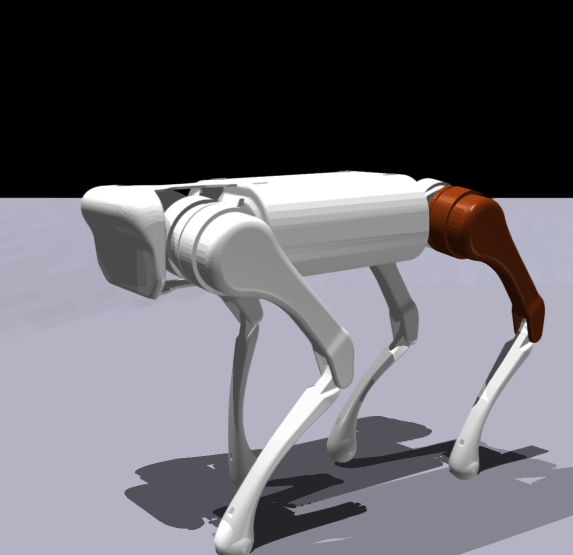
\includegraphics[width=\linewidth,trim=9bp 0bp 9bp 0bp,clip]{a1_robot_20261011_212425_original.png}\par
\small (a) Unitree A1
\end{minipage}\hfill
\begin{minipage}[b]{.48\columnwidth}
\centering
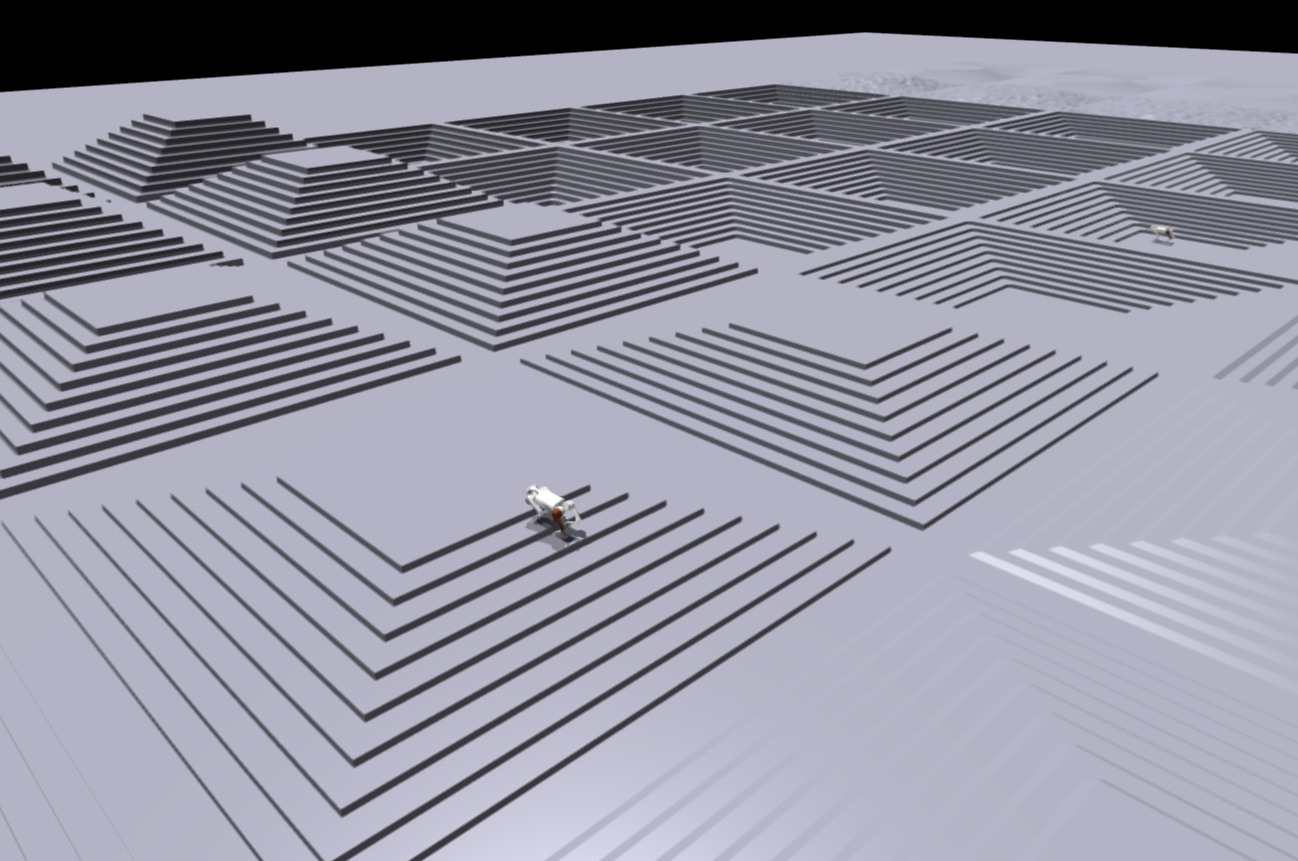
\includegraphics[width=\linewidth,trim=235 11 303 90,clip]{isaac_gym_original.png}\par
\small (b) Isaac Gym 지형
\end{minipage}
\caption{로봇 모델과 시뮬레이션 환경}
\label{fig:environment}
\end{figure}

\begin{table}[H]
\caption{로봇 및 제어 설정}\label{tab:system}
\centering\paperTableFont
\begin{tabularx}{\columnwidth}{@{}lY@{}}
\toprule
Parameter & Value \\
\midrule
Actuated joints & 12 (hip, thigh, calf per leg) \\
Physics / policy interval & 0.005 s / 0.02 s \\
Joint target & $q^{des}=q^0+0.25a_t$ (rad) \\
Nominal PD gains & $K_p=20$ N$\cdot$m/rad; $K_d=0.5$ N$\cdot$m$\cdot$s/rad \\
\bottomrule
\end{tabularx}
\end{table}


\subsection{단일 관절 토크 저하 모델}
토크 배율로 구동기 저하를 나타내는 모델\cite{ref6}을 단일 관절에 적용한다. 고장 이후 선택된 관절의 배율은 $\eta_j=1-d$, 다른 관절은 1이다. $d\in[0,1]$은 토크 손실률이며 $d=0.4$는 명목 출력의 40\% 손실을 뜻한다. PD 토크에 모터 강도 $m_j$와 고장 배율을 곱하고 관절 한계 토크로 포화한다.
\begin{align}
\tau_j^{PD}&=K_p(q_j^{des}-q_j)-K_d\dot q_j \\
\tau_j&=\mathrm{clip}(m_j\eta_j\tau_j^{PD},-\tau_j^{max},\tau_j^{max})
\end{align}
$m_j$는 고장과 별도로 [0.9, 1.1]에서 무작위화하며, 이는 명목 모터 강도의 $\pm10$\%에 해당한다. $d=1$에서는 능동 토크가 상실되며 수동 관절 운동은 유지된다.

공동학습에서는 에피소드마다 전체 12개 중 손상 관절과 0--100\%의 여섯 손실 수준을 무작위로 선택한다. 시작 후 2--10 s에 고장을 발생시키고, 이후 관찰 동안 해당 배율을 유지한다.


\section{교사·학생 공동학습 기반 보행 정책}

\subsection{관측 및 이력 표현}
현재 관측 $o_t$는 기존 보행 연구\cite{ref1}를 바탕으로 로봇·명령 관측 48차원과 지형 높이 187차원으로 구성된다(표~\ref{tab:observation}). 관절각은 기준 자세와의 차이이다. 표의 단위는 관측 스케일 적용 전 물리량이며, 중력 방향과 행동은 무차원이다.

\begin{table}[H]
\caption{현재 관측의 구성}\label{tab:observation}
\centering\paperTableFont
\begin{tabularx}{\columnwidth}{@{}Yccr@{}}
\toprule
Component & Symbol & Unit & Dim. \\
\midrule
Body linear velocity & $v_t$ & m/s & 3 \\
Body angular velocity & $\omega_t$ & rad/s & 3 \\
Projected gravity & $g_t$ & -- & 3 \\
Linear velocity command & $v_{xy}^{cmd}$ & m/s & 2 \\
Yaw-rate command & $\omega_z^{cmd}$ & rad/s & 1 \\
Relative joint position & $q_t-q^0$ & rad & 12 \\
Joint velocity & $\dot q_t$ & rad/s & 12 \\
Previous action & $a_{t-1}$ & -- & 12 \\
\midrule
Robot/command observation & $\tilde o_t$ & mixed & 48 \\
Terrain heights & $h_t$ & m & 187 \\
\midrule
Current observation & $o_t$ & mixed & 235 \\
\bottomrule
\end{tabularx}
\end{table}

\begin{table}[H]
\caption{교사·학생 인코더와 공유 Actor의 입출력}\label{tab:encoders}
\centering\paperTableFont
\begin{tabularx}{\columnwidth}{@{}>{\raggedright\arraybackslash}p{24mm}Y@{}}
\toprule
Path & Input $\rightarrow$ output \\
\midrule
Teacher encoder & Privileged information: $45\rightarrow z_t^T\in\mathbb R^8$ \\
Privileged components & Friction 1, mass 1, motor strength 12, PD gains 24, body velocities 6, fault flag 1 \\
Student encoder & $H_t=[\tilde o_{t-49},\ldots,\tilde o_t]$: $50\times48\rightarrow z_t^S\in\mathbb R^8$ \\
Training feature & $z_t=(1-\alpha)z_t^T+\alpha z_t^S$: 8 \\
Actor/Critic (training) & $[o_t,z_t]$: $235+8=243$ \\
Actor (inference) & $[o_t,z_t^S]$: $235+8=243\rightarrow a_t\in\mathbb R^{12}$ \\
\bottomrule
\end{tabularx}
\end{table}

학생의 시간 합성곱 인코더는 최근 50개 관측(약 1 s)에서 행동과 운동 반응의 관계를 추출한다\cite{ref4,ref3}. 없는 과거 표본은 0으로 채운다. 지형 높이는 이력에서 제외하고 현재 관측으로 Actor에 제공하며, 몸체 속도와 함께 시뮬레이터에서 획득한다.

\subsection{속도 추종 보상}
기존 병렬 보행 정책의 보상 구성\cite{ref1}을 바탕으로 평면 선속도와 yaw-rate의 추종 보상은 각각 다음과 같다.

\begin{equation}
r_v=\exp\left(-\|v_{xy}-v_{xy}^{cmd}\|_2^2/0.25\right)
\end{equation}
\begin{equation}
r_\omega=\exp\left(-(\omega_z-\omega_z^{cmd})^2/0.25\right)
\end{equation}
추종항과 보행 안정성을 위한 비용·보상항의 가중치는 표~\ref{tab:reward}와 같다. 각 항은 원시 물리량으로 계산하고, 가중합에 제어 간격을 곱한 뒤 음수 총보상을 0으로 제한한다. PPO\cite{ref5}로 할인 보상합을 최대화한다.


\begin{table}
\caption{제어 간격 적용 전 보상항별 가중치}\label{tab:reward}
\centering\paperTableFont
\begin{tabularx}{\columnwidth}{@{}Yl@{}}
\toprule
Reward term & Weight \\
\midrule
Planar velocity tracking / yaw-rate tracking & 1 / 0.5 \\
Squared vertical velocity & $-2$ \\
Squared roll/pitch angular velocity & $-0.05$ \\
Squared joint torque & $-2\times10^{-4}$ \\
Squared joint acceleration & $-2.5\times10^{-7}$ \\
Squared action change & $-0.01$ \\
Disallowed contact count & $-1$ \\
Joint-limit excess & $-10$ \\
Foot air-time reward & 1 \\
\bottomrule
\end{tabularx}
\end{table}

\subsection{교사·학생 공동학습}
교사 특징을 이력 기반 학생 특징으로 대체하는 구조\cite{ref3}와 특징 혼합 공동학습\cite{ref4}을 적용한다. 모방 오차가 남아도 정책이 학생 특징으로 보행을 학습하도록, 두 특징을 혼합해 Actor 및 Critic에 입력한다.

\begin{equation}
z_t=(1-\alpha)z_t^T+\alpha z_t^S
\end{equation}
사전학습 교사로 초기화하고 공동학습 10,000회 동안 $\alpha$를 0에서 1까지 선형 증가시킨다. 전환 중에는 PPO 손실에 모방항을 추가한다.

\begin{equation}
\mathcal L=\mathcal L_{PPO}+\frac{1-\alpha}{B}\sum_{i=1}^{B}\|z_i^S-\mathrm{sg}(z_i^T)\|_2
\end{equation}
혼합 스케줄과 손실은 선행 연구\cite{ref4}를 따른다. $B$는 미니배치 크기, $\mathrm{sg}$는 모방 목표의 gradient 차단 연산이다. 교사는 PPO 경로로 갱신하며 $\alpha$=1 이후에는 학생·Actor·Critic를 학습한다. 병렬 환경 4,096개, 할인율 0.99, GAE 계수 0.95, PPO clip 계수 0.2를 사용하였다. 입력 경로와 특징 혼합은 그림~\ref{fig:architecture}에 나타내었다.

\begin{figure}[H]
\centering
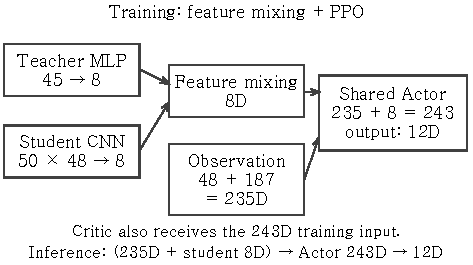
\includegraphics[width=\columnwidth]{paper_workflow_v8.pdf}
\caption{교사·학생 특징 인코딩과 공동학습 및 추론 구조}\label{fig:architecture}
\end{figure}

\section{시뮬레이션 결과 및 평가}

\subsection{평가 조건과 지표}
정상 조건에서 학습한 정책(Normal)과 교사·학생 공동학습을 거친 학생 정책(Student)을 비교하였다. 두 정책은 각각 seed 1로 학습하였으며, 평가에서는 초기 물리 조건·지형·고장 일정을 동일하게 설정하였다.

\begin{table}
\caption{정책 비교를 위한 평가 조건}
\centering\paperTableFont
\begin{tabularx}{\columnwidth}{@{}lY@{}}
\toprule
Item & Setting \\
\midrule
Command & $v_x$=0.5 m/s; $v_y$=$\omega_z$=0 \\
Conditions & 12 joints $\times$ d$\in$\{0,.2,.4,.6,.8,1\} \\
Onset / observation & 2–10 s / 20 s after onset \\
Trials & Evaluation seeds 301–303 $\times$ 16; 48 per joint/loss \\
Failure & Base contact force >1 N; pre-fault failure included \\
\bottomrule
\end{tabularx}
\end{table}
혼합 지형과 물리 무작위화는 유지하고 관측 잡음·외부 밀기·curriculum은 해제하였다. 생존율은 고장 전 실패를 포함한 전체 시행 중 종료 시 생존한 비율이다. 명령 추종 오차는 고장 후 생존 구간의 속도 표본 $K$개로 계산하였다.

\begin{equation}
\mathrm{RMSE}_u=\sqrt{\frac{1}{K}\sum_{k=1}^{K}(u_k-u^{cmd})^2}
\end{equation}
여기서 $u\in\{v_x,v_y,\omega_z\}$이며 각 명령은 0.5 m/s, 0 m/s, 0 rad/s이다. 명령 추종 시간율 $Q_{20}$은 |$v_x$−0.5|$\leq$0.1 m/s, |$v_y$|$\leq$0.1 m/s, |$\omega_z$|$\leq$0.2 rad/s를 동시에 만족한 생존 시간을 고장 후 전체 20 s로 나눈 값이다. 전진속도 허용오차는 명령의 20\%이며, 낙상 이후 시간은 조건을 만족하지 않은 시간으로 포함한다. 엄격 추종률 $Q_{10}$은 각 허용오차를 절반으로 설정한다.

고장 후 실제 이동량은 전방 순변위 $D_\parallel$로 평가하였다. 고장 순간과 마지막 생존 표본의 세계좌표 xy 변위를 고장 순간의 수평 전방 $\hat u^f$에 투영하였다.
\begin{equation}
D_{\parallel}=(x^{last}-x^f)^\top\hat u^f
\end{equation}
고장 전 종료된 시행의 $D_\parallel$는 0으로 처리하였다.


\subsection{학습 과정}
\begin{figure}
\centering
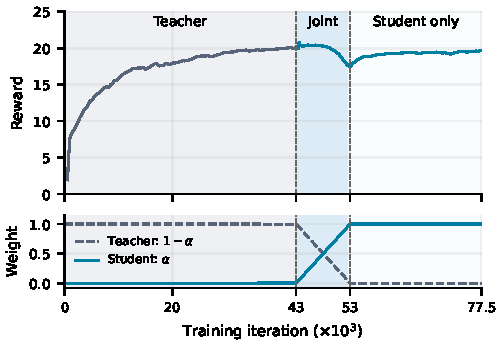
\includegraphics[width=\columnwidth]{paper_learning_v10.pdf}
\caption{학습 단계별 평균 에피소드 보상(상단, 500회 이동평균)과 교사·학생 특징의 혼합 비중(하단)}\label{fig:learning}
\end{figure}
그림~\ref{fig:learning}은 평균 에피소드 보상과 특징 혼합 비중을 나타낸다. 교사를 43,000회까지 학습한 후 공동학습을 초기화하였다. 43,000--53,000회에는 학생 비중 $\alpha$를 0에서 1로 증가시키고, 이후 학생 특징만 사용하였다.

학생 특징으로 전환되는 동안 감소한 보상은 학생 단독 학습에서 회복하였다. 전환 시점과 최종 평균 보상은 각각 17.52와 19.70으로 12.4\% 증가하였다.


\subsection{토크 저하에 따른 생존 및 명령 추종 성능}
\begin{figure}
\centering
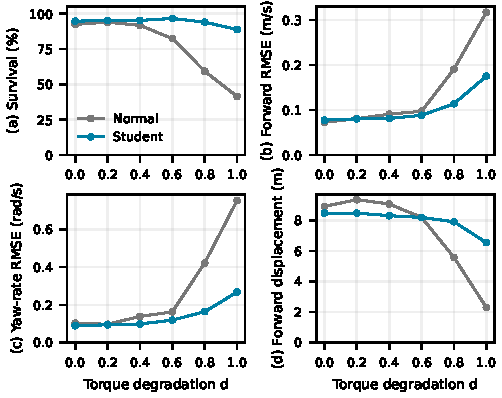
\includegraphics[width=\columnwidth]{paper_metrics_v10.pdf}
\caption{토크 손실에 따른 생존율, 전진속도·yaw-rate 추종 오차 및 전방 순변위}\label{fig:performance}
\end{figure}
그림~\ref{fig:performance}에서 강한 토크 저하에 따른 Student의 생존율 향상과 전진속도·yaw-rate 오차 감소가 함께 나타났다.

\begin{table}
\caption{정책별 성능 차이(Student−Normal)}\label{tab:performance_gain}
\centering\paperTableFont
\setlength{\tabcolsep}{2pt}
\begin{tabularx}{\columnwidth}{@{}>{\centering\arraybackslash}p{7mm}*{4}{>{\centering\arraybackslash}X}@{}}
\toprule
손실\newline (\%) & 생존율\newline (\%p) & $v_x$ RMSE\newline (m/s) & yaw RMSE\newline (rad/s) & 전방 변위\newline (m) \\
\midrule
0 & +2.26 & +0.0047 & -0.0133 & -0.437 \\
20 & +1.22 & -0.0003 & -0.0027 & -0.881 \\
40 & +3.47 & -0.0094 & -0.0399 & -0.766 \\
60 & +14.24 & -0.0090 & -0.0437 & -0.004 \\
80 & +34.72 & -0.0767 & -0.2578 & +2.333 \\
100 & +47.40 & -0.1418 & -0.4850 & +4.250 \\
\bottomrule
\end{tabularx}
\end{table}
표~\ref{tab:performance_gain}의 생존율 차이는 양수일수록 생존율 증가를, 두 RMSE 차이는 음수일수록 추종 오차 감소를 나타낸다. 전방 변위 차이는 고장 이후 실제 이동량의 차이이며, 생존 및 명령 추종과 함께 해석한다.

\subsection{관절별 고장 대응 성능}
\begin{figure}
\centering
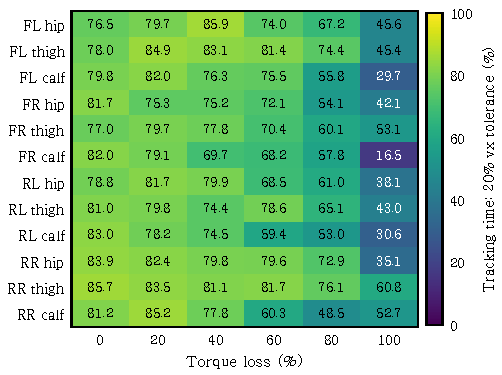
\includegraphics[width=\columnwidth]{paper_joint_tracking20_v12.pdf}
\caption{관절 및 토크 손실별 Student 명령 추종 시간율 $Q_{20}$(\%)}\label{fig:joint_tracking}
\end{figure}
FL/FR은 좌/우 앞다리, RL/RR은 좌/우 뒷다리이다. 그림~\ref{fig:joint_tracking}은 3축 속도 허용오차를 동시에 만족한 시간을 비교한다. 완전 손실에서 RR thigh는 60.84\%, FR calf는 16.49\%로 관절별 차이가 나타났다. FR calf의 생존율은 83.33\%였으나 전진속도와 yaw-rate RMSE는 각각 0.256 m/s와 0.382 rad/s였다. 생존을 유지한 이후에도 손상 관절에 따라 명령 수행의 취약성이 다르게 나타났다.



\section{결론 및 향후 연구}
교사·학생 공동학습을 단일 관절 토크 저하에 적용한 4족 보행 정책을 구성하였다. 완전 손실에서 생존율은 Normal 41.49\%에서 Student 88.89\%로 증가하고, 전진속도·yaw-rate RMSE는 각각 0.317→0.175 m/s, 0.753→0.268 rad/s로 감소하였다. 관절별 추종 시간율은 생존 이후의 명령 수행 취약성을 구분하였다.

향후 여러 관절의 동시 토크 저하와 관절 잠금 고장으로 적용 범위를 확장하고, 고장 유형과 손상 조합에 따른 보행 안정성 및 속도 추종 성능을 평가할 예정이다.

\begin{thebibliography}{9}
\paperreferencefont
% 좁은 단에서 영문 참고문헌의 단어 간격이 벌어지지 않도록 왼쪽 정렬한다.
\raggedright
\bibitem{ref1} N. Rudin et al., “Learning to Walk in Minutes Using Massively Parallel Deep Reinforcement Learning,” PMLR 164, pp.91–100, 2022.
\bibitem{ref4} D. Liu et al., “Saving the Limping: Fault-tolerant Quadruped Locomotion via Reinforcement Learning,” arXiv:2210.00474v3, 2023.
\bibitem{ref2} V. Makoviychuk et al., “Isaac Gym: High Performance GPU-Based Physics Simulation for Robot Learning,” arXiv:2108.10470, 2021.
\bibitem{ref6} X. Wu et al., “Adaptive Control Strategy for Quadruped Robots in Actuator Degradation Scenarios,” DAI 2023, doi:10.1145/3627676.3627686.
\bibitem{ref3} A. Kumar et al., “RMA: Rapid Motor Adaptation for Legged Robots,” RSS XVII, 2021, doi:10.15607/RSS.2021.XVII.011.
\bibitem{ref5} J. Schulman et al., “Proximal Policy Optimization Algorithms,” arXiv:1707.06347, 2017.
\end{thebibliography}
